\section*{Research Design}

The empirical analyses presented below use the country-year as the unit of analysis. Our sample includes all countries that are independent members of the international system between July 2002, when the ICC became active, and the end of 2016. We include all country-years in our main analysis, rather than a restricted sample of countries, because the potential for ICC involvement is theoretically global: non-states parties can be referred by the UNSC (e.g. Libya), can adopt ICC jurisdiction voluntarily (e.g. Ukraine), or can fall under the court's jurisdiction as a result of military intervention on the territory of ratifier states (e.g. United States). However, recognizing that the probability of ICC involvement is likely substantially lower for countries with strong human rights records and no recent history of political violence, and that the pathways to ICC involvement for countries that are non-ratifiers of the Rome Statute are much more restricted, we present two additional analyses in the supplementary materials that restrict the sample to (1) countries that have experienced political terror (PTS) scores of 3 or higher or have experienced civil conflict since 2002, and (2) ICC ratifier states.\footnote{One alternative would be to restrict the sample to the set of situations that have been referred to the OTP through communications from states, international organizations, non-governmental organizations, and individuals. The OTP does not make details on communications publicly available, however, so it is not possible to build a sample for analysis based upon actual communications to the court.}

\subsection*{Response Variables}

The empirical analyses test the determinants of moving from no ICC involvement, to a preliminary examination, and then to a formal investigation, while also accounting for the target (government or opposition) of the ICC's involvement. Specifically, we examine two sequentially ordered dependent variables:

\begin{itemize}
	\item State-Focused ICC Involvement
	\item Opposition-Focused ICC Involvement
\end{itemize}

To measure these variables, we need to determine what countries the ICC gets involved in and who, within those countries, the OTP targets in its examinations and investigations. Because the OTP examines and investigates \textit{situations}, rather than countries or specific actors, determining who the OTP targets is non-trivial. To do this, we researched each situation that the OTP has examined or investigated since the ICC became active in 2002 (through 2016). For each situation, we first determined which country or countries were the focus of the OTP's activities. We considered a particular country to be under examination/investigation if actions taken by officials or nationals of that country were \textit{explicitly} being examined or investigated by the ICC. Evidence of explicit examination or investigation includes explicit references to the behavior of or crimes potentially committed by government/nationals of that country in ICC reports and documentation. We examined a variety of documents from the ICC, including press releases on the opening of examinations/investigations, annual reports on the Court's activities, summary reports for ongoing cases, etc. Importantly, our coding rules mean that the state associated with a particular ``situation'' in the ICC's documentation is not necessarily the state, or the only state, experiencing ICC involvement. For example, the situation referred to the ICC by Comoros, Greece, and Cambodia does not involve an investigation of actions taken by these states or their nationals, but instead is focused on potential abuses committed by the Israeli government. We therefore treat Israel as the target of ICC involvement, while excluding Comoros, Greece, and Cambodia as ICC targets. Additionally, in the court's preliminary examination focused on Afghanistan, both Afghanistan and the United States are implicated. This is because reports provided by the ICC on it's preliminary examination activities explicitly refer to potential abuses perpetrated by Afghan forces and nationals, as well as to potential abuses committed by US forces in Afghanistan. Thus, ICC involvement is coded for both Afghanistan and the United States.

After identifying which states have been targeted by OTP examinations and investigations, we then determined whether the OTP targeted government and/or opposition actors in each of the target countries. We consider the ICC's actions to be government-targeting if they involve examining/investigating actions taken by current members of the state's security forces or current political leaders. We also consider actions to be state-targeting if the Court investigates alleged crimes committed by supporters of or groups supported by the current regime.\footnote{For example, this includes crimes allegedly committed on behalf of Kenyan government officials by private citizens (i.e. lawyers engaging in witness tampering on their behalf). This would also include crimes allegedly committed by pro-government militia groups that receive state backing.} We consider the OTP's actions to be opposition-targeting if they focus on current rebel group members, political opponents of the current regime, or any other actors who are not considered state targets. In several cases, both state and opposition figures are implicated in the OPT's investigations. In these cases, both state-focused and opposition-focused OTP investigations are recorded in our data. For example, according to court documents, the OTP's preliminary examination into the situation in Colombia explicitly focuses on actions taken by rebel organizations (i.e. FARC and ELN), pro-government paramilitaries, and the state's own security forces. Therefore, both \emph{State-Focused ICC Involvement} and \emph{Opposition-Focused ICC Involvement} are coded 1 from 2004, when the examination began, through 2016, as both state officials/agents and members of opposition groups are potentially implicated.

After identifying which government and non-state actors have been the focus of ICC involvement, we code the level of ICC involvement targeting those actors in any given year. Our resulting dependent variables, \emph{State- and Opposition-Focused ICC Involvement}, measure the level of ICC involvement in a given year on a scale from 0 to 2. For both variables, we code the highest level of ICC involvement reached in any given year that is focused on a current member or supporter of the government (state-focused) or opposition (opposition-focused). The levels of ICC involvement are as follows: 0 if there is no ICC involvement, 1 if the highest level of ICC involvement in the current year is a preliminary examination (proprio motu authority cases) or pre-investigation phase (state and UNSC referral cases), and 2 for years in which a formal investigation is ongoing. This last category includes cases that have progressed to the issuing of warrants or summons and ongoing trials).\footnote{We do not distinguish between stages after a formal investigation because of the small number of cases that have advanced to that point.} For example, Sudan is coded as having no ICC involvement prior to March 2005. From March 2005 through May 2005, ICC involvement is coded 1, as the UNSC had referred the case to the ICC and the OTP was engaged in a pre-investigation phase analysis of information. From June 2005 through December 2016, Sudan receives a coding of 2 for both state- and opposition-focused ICC involvement, as a formal investigation targeting both government and opposition figures was ongoing. Figure \ref{fig:iccMaps} below provides an easy visualization of the highest level of state-focused and opposition-focused ICC involvement reached for each country between 2002 and 2016.

It is important to note that ICC involvement proceeds through these stages sequentially. That is, cases always begin with no ICC involvement, and the OTP always then engages in a preliminary or pre-investigation examination before reaching the formal investigation stage. As we discuss in more detail below, traditional ordinal regression approaches are inappropriate given the sequential nature of our DV, and we therefore introduce an approach that accounts for transitions between the sequentially ordered stages. It is also important to note that our dependent variables are coded based upon the status of those being investigated in any given year. This means that the level of state or opposition-focused ICC involvement may change if the status of those under investigation changes. This can occur, for example, if a regime change occurs in which targeted government officials lose power or targeted opposition members come to power.\footnote{For example, the ICC investigation into the situation in Libya began as a state-focused investigation, as the OTP's efforts were focused on current state officials - Gaddafi and members of his inner circle. This changed, however, in September 2011, when the Gaddafi regime fell and former regime opponents took power. At that point, we code the ICC's involvement as opposition-focused. In this and one other case where similar side-switching occurs (DRC), we restrict the ICC involvement coding to 1 in the first year after the switch to avoid violating model assumptions.}

Based upon the above coding rules, \emph{State-Focused ICC Involvement} is coded 0 in 2,786 observations (96\%), 1 in 90 observations (3\%), and 2 in 30 observations (1\%). \emph{Rebel-Focused ICC Involvement} is coded 0 in 2,775 observations (95\%), 1 in 66 observations (2\%), and 2 in 65 observations (2\%).

\begin{figure}
    \centering
    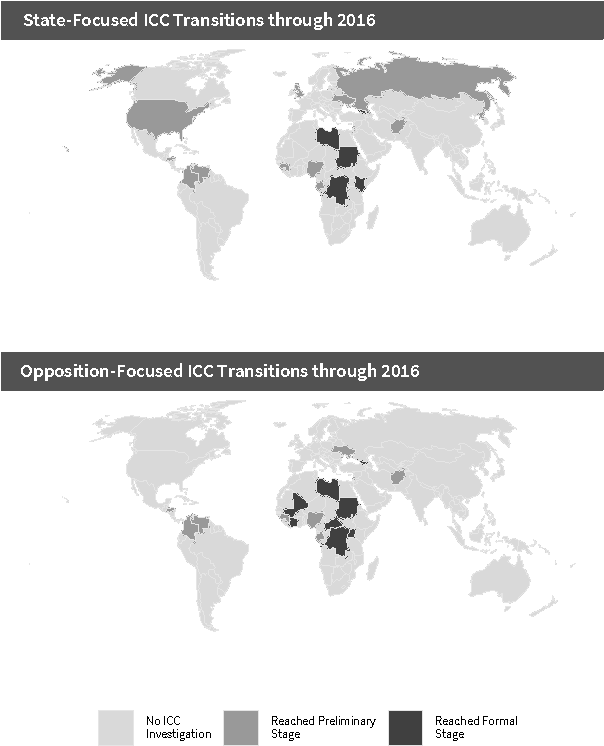
\includegraphics[width=1\textwidth]{iccMaps.pdf}
    \caption{Caption}
    \label{fig:iccMaps}
\end{figure}
\FloatBarrier

\subsection*{Impartiality Variables}

To test the expectation that concerns over impartiality will drive the OTP's target selection, we include variables that capture the gravity of human rights abuses and the likelihood of effective domestic accountability. First, we use the Uppsala Conflict Data Program's (UCDP) Georeferenced Event Dataset (GED) to identify the number of civilians killed by government and opposition groups in any given year \citep{sundberg2013introducing}. The GED is an events dataset that includes information on all instances of intentional civilian targeting, or One Sided Violence (OSV), perpetrated by governments and nongovernmental actors since 1989. It is important to acknowledge that the GED data capture only OSV, and therefore do not encompass all types of violations of international humanitarian law (IHL) that might fall within the ICC's jurisdiction. Despite this limitation, intentional civilian killing is an appropriate measure because the extrajudicial killing of noncombatants is expressly prohibited by IHL \citep{blank2018international}.

Further, these data are ideally suited for this study because they enjoy several advantages over potential alternative measures. First, they are available through 2016, whereas many other existing datasets that capture broader human rights practices end earlier, which would force us to shorten our analysis timeframe and ignore important cases of ICC involvement. Second, these data allow us to identify the perpetrators of human rights violations. Other possible datasets such as PTS and CIRI provide only a single country-level `score', which identifies the level of human rights violations in a given country. They do not allow us to identify violations perpetrated by non-state actors, as the scores generally refer to state-based abuses only. This is critically important, given that ICC action is often directed at specific non-state or opposition actors, not at the state itself, and hypothesis 1 predicts that the identity of the perpetrator of human rights violations matters for who the OTP targets. Finally, the OSV data provided by GED provides several advantages over alternatives because it is measured at the event-level. It can therefore be easily aggregated to generate a measure of the magnitude of OSV perpetrated by government or non-state actors in a given year. %Other human rights datasets, which tend to provide yearly summary measures of human rights violations, provide less variation and are not as compatible with our monthly data on ICC involvement.

% However, we do acknowledge that this is an imperfect solution, as the OSV data are measured at the yearly level, and we therefore must make assumptions about how deaths from a given year are split across months (i.e. equally). Other data sources have more micro-level civilian deaths data for Syria, but these are not ideally suited for combining with GED because the definition of OSV is not the same across other data sources, whereas the two UCDP dataset use the same definition of civilian targeting.
To measure government OSV, we first generate the sum of all civilians killed in one-sided violence events perpetrated by each government in a particular year based upon the raw events data from GED.\footnote{The GED does not include data for Syria, but otherwise has global coverage. We therefore include data from UCDP's One-Sided Violence dataset \citep{eck2007one} for Syria, which allows us to include Syria, a potentially important case, in our analysis. Our results remain consistent if we exclude Syria from the analysis.} We then generate a running sum of the number of civilians killed in government-perpetrated OSV since July 2002 through the current year. This running sum provides a measure of the magnitude of human rights violations perpetrated by the state since the ICC became active. It is important to use this running sum rather than a simple measure of deaths in the current year because the OTP can decide to investigate instances of war crimes or crimes against humanity that occurred any time since a state came under its jurisdiction or since the court became active (if referred by the UNSC or the state itself), and because OTP examinations/investigations are generally retroactive rather than simply reflecting current violations.\footnote{An alternative would be to create a running sum of OSV perpetrated since the state became a ratifier of the Rome Statute. However, this would not allow us to include states that have not ratified the Rome Statute, and would ignore the fact that states can come under investigation by the ICC for crimes committed despite non-ratification if they are referred by the UNSC, are a non-state party who accepts the Court's jurisdiction on an ad hoc basis, or commit crimes on the territory of a ratifier state.} In our analysis predicting State-Focused ICC Involvement, we include the natural log of the running sum of state-perpetrated OSV since July 2002, and lag this value one year. This variable ranges from 0 to 8.69, with a mean of 0.979. Finally, we allow the effect of this variable to vary across values of the DV, rather than forcing its effect to be stable when predicting the onset of an examination and the transition to a formal investigation.

Measuring opposition-perpetrated OSV required us to first identify the set of relevant actors within each country. Because rebel groups, terrorists, and other non-state perpetrators of OSV can cross international borders and engage in civilian targeting in more than one state, we could not simply associate each non-state OSV perpetrator in the GED dataset with a single state. Instead, we used information provided by GED on the \textit{location} of each OSV event to determine on which country's territory the event took place. This is important because the location of OSV is relevant for determining jurisdictional issues, as OSV perpetrated on the territory of a state party to the Rome Statute falls within the OTP's jurisdiction, and that perpetrated on the territory of a non-state party may not. Once we identified all OSV events perpetrated by non-state actors on the territory of a given state in a given year, we summed the resultant deaths to create a yearly total of civilians killed by non-state actors in that country-year. We then generated a running sum of the number of civilians killed in opposition-perpetrated OSV since July 2002 through the current year, analogous to the measure used for state-perpetrated OSV. In our models predicting Opposition-Focused ICC Involvement, we include the natural log of the running sum of opposition-perpetrated OSV since July 2002, lagged one year. This variable ranges from 0 to 9.41 with a mean of 1.19. Again, we allow this variable's effect to vary across values of the DV.

Finally, to proxy the likelihood that a state is willing and able to hold perpetrators accountable via domestic judicial processes (H2), we include a measure of judicial independence from the Varieties of Democracy (V-Dem) project \citep{coppedge2018v}. Domestic judicial independence is a useful proxy for complementarity because it captures the likelihood that domestic judiciaries are willing and able to investigate alleged perpetrators of war crimes and crimes against humanity. States with strong, independent judiciaries have the capacity to investigate perpetrators, while those with weak, non-independent judiciaries cannot credibly threaten an independent, effective investigation or trial. This holds for investigations that target both the state and opposition: a non-independent judiciary will be unable to hold state officials accountable because the judiciary is dependent upon those state officials. Similarly, a non-independent or weak judiciary will be unable to carry out an effective, unbiased investigation of opposition perpetrators either because of state interference or lack of resources and enforcement power. States with strong judiciaries, therefore, make both state-focused and opposition-focused ICC involvement less necessary. It is important to note that while this is a useful proxy for complementary domestic accountability, it is an imperfect one. Judicial independence should increase the likelihood of impartial, effective domestic judicial processes, but does not automatically mean that domestic courts will hold perpetrators accountable. Lacking more precise measures of complementarity for the time period under examination, we use judicial independence to proxy our concept of interest.\footnote{Importantly, judicial independence does positively correlate with human rights trials in available data: we regress human rights trials on our measure of judicial independence while controlling for regime-type, physical integrity violations, one-sided violence, regional prosecutions, and a lagged response variable. Data on trials and controls come from \citet{dancy2019behind}. We find that judicial independence is a significant predictor of trials, which supports our claim that judicial independence is related to domestic accountability. We cannot use the actual trials data in our analysis because it is available only through 2010 and only for post-transition countries, which would limit our sample significantly.} Specifically, we include a measure of lower court judicial independence from V-Dem \citep{coppedge2018v}. We prefer V-Dem's lower court rather than high court independence measure because lower courts are the predominant location for domestic human rights prosecutions. Descriptive data available from the Transitional Justice Research Collaborative website, for example, indicates that over 80\% of domestic human rights trials between 2002 and 2010, for which court information was available, involved lower courts.\footnote{Information available at: https://www.transitionaljusticedata.com/.} Higher values of this measure indicate greater independence of a state's judiciary.\footnote{The specific question asked in the V-Dem survey is: ``When judges not on the high court are ruling in cases that are salient to the government, how often would you say that their decisions merely reflect government wishes regardless of their sincere view of the legal record?''. The surveys asks this question of respondents on an ordinal scale (0-4) and then combines responses using a measurement model.} This variable is lagged one year because it is measured at the yearly level, and ranges from -3.19 to 3.43 with a mean of 0.346. We also model this variable to allow differential effects on the transition between stages of the ICC process.

\subsection*{Powerful States' Interests Variables}

To test the expectation that concerns over powerful states' interests will drive the OTP's target selection, we include two variables that capture the closeness of potential target countries to the P5: foreign policy ideal point distance and an Africa dummy. First, we generate a measure of foreign policy preference similarity between a given state and the P5 using data on countries' foreign policy ideal points from \citet{bailey2017estimating}. For each state in our dataset, we measure the absolute value of the distance between that state's ideal point and each of the P5's ideal points. We retain the minimum of the five values generated as our measure of that country's minimum ideal point distance to the P5. In other words, this variable captures each country's ideal point distance from the closest of the P5 states. Higher values indicate greater distance, or greater policy preference dis-similarity, while lower values indicate increasing closeness. Each of the P5 is assigned a value of zero, as each P5 state's minimum ideal point distance to itself is always zero. This allows us to capture the fact that P5 states are most likely to want to avoid ICC examinations and investigations of their own behavior, above and beyond their desire to avoid ICC targeting of countries with which they share close ties. The resulting measure, therefore, is inversely related to P5 closeness: as minimum ideal point distance increases, the state in question gets farther and farther from the P5 in terms of policy similarity. Our theoretical expectation is that as this distance increases, the P5 have less of a vested interest in the internal politics of that state, P5 interests will therefore be less threatened by ICC involvement, and the likelihood of ICC examinations and investigations increases. This measure is lagged 1 year, as it is measured at the yearly level. It ranges between 0 (coded for each of the P5) and 1.37, with a mean of 0.307. We model this variable to allow differential effects across the preliminary examination and formal investigation stages of ICC involvement.

Second, we include a binary variable to account for whether the state is in Africa. This variable is a useful proxy for P5 interests, given that some argue that the OTP disproportionately targets African states because they lack strong links with major powers that can shield them from the Court \citep{arieff2010international, hoile2014justice, rudolph2017power}. Indeed, as \citet[26]{arieff2010international} argue, ``some commentators allege that the Prosecutor has limited investigations to Africa because of geopolitical pressures, either out of a desire to avoid confrontation with major powers or as a tool of Western foreign policy." We thus see a clear link between the Africa bias discussed above, and powerful states' interests, and expect that if P5 geopolitical interests are driving OTP decision-making, the ICC will be more likely to target African governments and non-state actors at both the preliminary examination and formal investigation stages. This variable equals 1 if the country is on the African continent, and zero otherwise. It is coded one in 9,288 of 33,706 observations (28\%). To get a more nuanced understanding of the Africa bias, we model this variable by allowing differential effects across stages of ICC involvement.

It is important to acknowledge that these two variables are relatively blunt proxies for P5 interests in a given country. Arguably, there are other ways we might conceptualize and measure ties to P5 states, such as alliance ties or P5 military intervention. These alternatives are limited in several ways, however, that make them unsuitable for use in our analyses. First, data on P5 military interventions are not available for most of the time period covered by our analysis, so cannot be included (e.g. the International Military Interventions data \citep{pickering2009international} are available only through 2005). Alliance ties data are available for more of our time period, but provide a largely static measures that is unable to account for dynamic relationships with P5 states. Specifically, once states form alliances, they tend to remain allies for a significant period of time \citep{leeds2007terminating}. Measuring P5 interests via alliance ties, therefore, would mask changes in P5 closeness that do not rise to the level of forming or abrogating alliance ties, and would thus provide only a blunt measure of cross-sectional variation. A similar limitation applies to trade agreements data, another potential measure of P5 interests. We therefore focus on the above two variables. The UNGA voting data that is used to create the ideal point distance measure is better able to capture less drastic, yet still important, temporal and cross-sectional variation in countries' ties to the P5. And while Africa is a static measure that captures only cross-sectional variation, it is valuable in that it both captures P5 interests, broadly speaking, and also allows us to directly speak to the claims of Africa bias leveled against the ICC.


\subsection*{Control Variables}

We also include several potential confounders as control variables in the analysis. First, we control for whether the state in question ratified the Rome Statute. Ratifying the Rome Statute gives the ICC jurisdiction over the state in question and its nationals, so is likely to increase the chances of ICC involvement.\footnote{As noted above, ratification is not a prerequisite for ICC involvement, but is still likely to increase its likelihood.} Ratification may also be correlated with key variables of interest, particularly our measure of human rights violations, if states use ratification as a signal to demonstrate their commitment to peace \citep{simmons2010credible}. ICC Ratification is a binary variable coded 1 in the year a state ratified the Rome Statute, and in all subsequent years. This variable is coded 1 in 19,028 observations (56\%). Data were obtained from the ICC website.\footnote{\url{http://www.icc-cpi.int/EN\_Menus/icc/Pages/default.aspx}}

Second, we include a dummy variable to account for whether there is an ongoing civil conflict in the state, using the UCDP Armed Conflict Dataset \citep{themner2012armed}. We expect ICC involvement to be more likely if a civil war is ongoing. While the ICC is not responsible for prosecuting conflict per say, it is likely that the prevalence of conflict is correlated with war crimes. Further, civil conflict may be related to several of our key IVs, as conflict settings may be more likely to experience OSV, to be associated with low judicial independence and P5 affinity, and occur more frequently in Africa. This variable is lagged one year, and is coded 1 in 4,356 observations (13\%).

Third, we include polity2 scores as a measure of regime type \citep{marshall2018polity}. We expect the ICC to be less likely to become involved in situations in more democratic states, as these states likely have the resources and willingness to address human rights violations directly by holding human rights trials domestically \citep{kim2010explaining, herz1982dictatorship}, and are also likely to have better human rights records to begin with \citep{davenport:armstrongii:2004, davenport2007state}. At the same time, better human rights records and more trials (i.e. complementarity) are likely to deter ICC involvement. Models include the full polity scale ranging from 1 to 21, with a mean of 15.3 in our sample. This measure is lagged one year.
%need to check kim cite.

Finally, we also include a measure of economic development in the models, operationalized as the natural log of GDP per capita (2010 constant US dollars) from the \citet{world2018world}.  Economic development may have differential effects on both our theoretical variables of interest and our response variables. Wealthier countries with higher levels of infrastructure (e.g. roads) and bureaucracy may be more attractive places for the OTP to become involved because she can expect to be more effective in situations with relatively easier and greater access. In contrast, it is possible that developed states with greater political and legal resources may be able to deter ICC involvement. At the same time, economic development is related to the human rights practices of states \citep{hill:jones:2014} and human rights prosecutions \cite{kim2012structural}, and is positively correlated with P5 interests and strongly negatively correlated with our Africa dummy. Therefore, while there are different pathways for the impact of GDP, is is nonetheless an important variable to include in the models due to its relationship with several important independent variables and ICC involvement. This variable ranges from 5.27 to 11.88, with a mean of 8.43. It is lagged on year in the analyses.
% it said we used GDP, but I think it might be GDP per capita?  I'm not sure- variable name say gdpcap, which makes me think its per capita?

For each of these controls, we estimate a single, global coefficient, rather than stage specific effects across categories of our dependent variables. We do this because we do not have strong theoretical expectations that the effects of these variables should vary across stages. Further, because of the sparse nature of our dependent variables, particularly at the second stage, we simply do not have enough data for the model to ascertain well-behaved results when estimating stage-specific coefficients for all variables. Setting stronger priors could help address this issue, but we prefer to err on the side of conservative priors and stage-specific coefficients only for theoretical variables of interest.
% BA and SM should read this paragraph and edit as necessary - i basically just paraphrased what SM said in his email.
